\documentclass[border=10pt]{standalone}
\usepackage{tikz}
\usepackage{amsmath}
\usetikzlibrary{arrows.meta, positioning, fit, backgrounds, calc}

\begin{document}
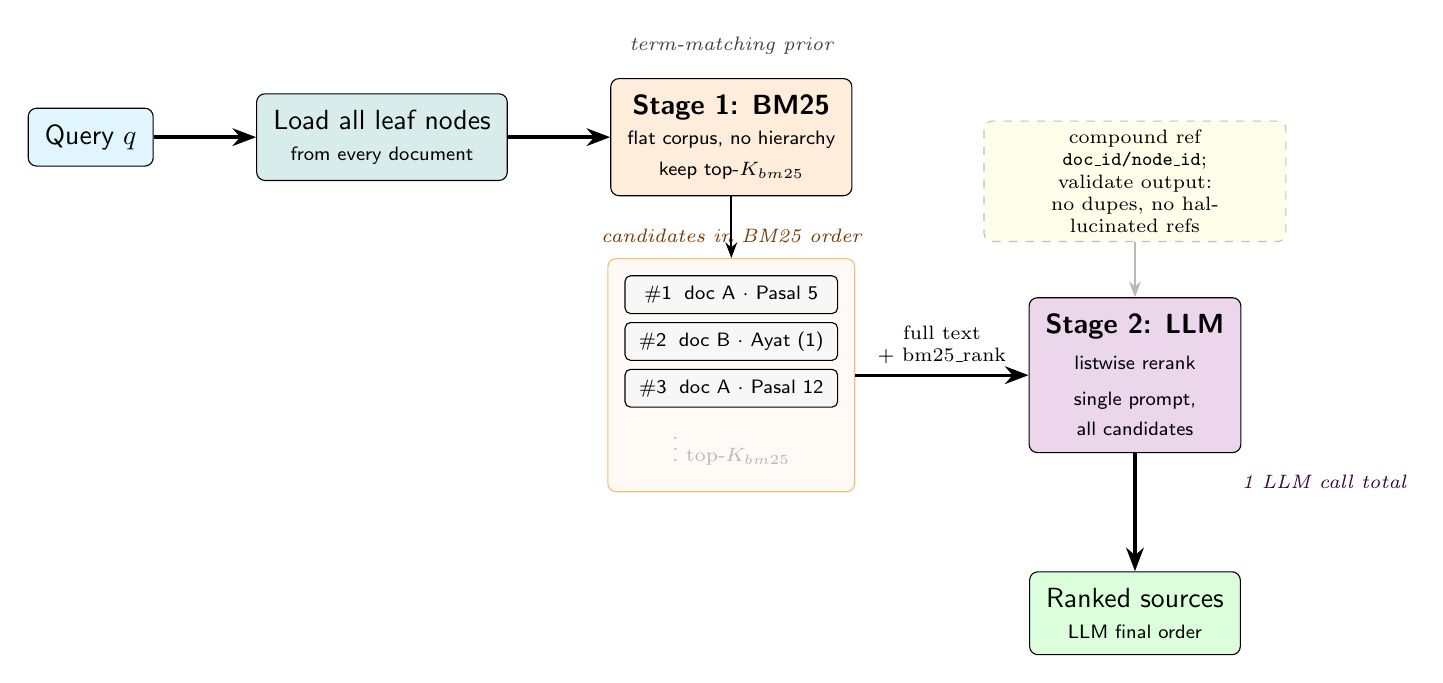
\begin{tikzpicture}[
    font=\small,
    box/.style={draw, rounded corners=3pt, align=center, font=\sffamily,
                inner sep=6pt},
    cand/.style={draw, rounded corners=2pt, minimum width=2.7cm, minimum height=0.48cm,
                 font=\scriptsize\sffamily, align=left, inner sep=3pt, fill=gray!6},
    flow/.style={-{Stealth[length=3mm]}, very thick},
    arr/.style={-{Stealth[length=2mm]}, semithick},
]

    %==================== QUERY ====================
    \node[box, fill=cyan!12] (q) {Query $q$};

    %==================== LOAD ALL LEAVES ====================
    \node[box, fill=teal!15, right=1.3cm of q, align=center] (load)
        {Load all leaf nodes\\[-1pt]{\scriptsize from every document}};
    \draw[flow] (q) -- (load);

    %==================== STAGE 1: BM25 over flat corpus ====================
    \node[box, fill=orange!14, right=1.3cm of load, align=center] (bm25)
        {\textbf{Stage 1: BM25}\\[-1pt]{\scriptsize flat corpus, no hierarchy}\\[-1pt]
         {\scriptsize keep top-$K_{bm25}$}};
    \draw[flow] (load) -- (bm25);

    \node[font=\scriptsize\itshape, text=gray!50!black, above=0.18cm of bm25]
        {term-matching prior};

    %==================== BM25-ranked candidate list ====================
    \node[cand] (c1) at ($(bm25.south)+(0,-1.25)$) {\#1\; doc A $\cdot$ Pasal 5};
    \node[cand, below=0.1cm of c1] (c2) {\#2\; doc B $\cdot$ Ayat (1)};
    \node[cand, below=0.1cm of c2] (c3) {\#3\; doc A $\cdot$ Pasal 12};
    \node[font=\scriptsize, text=gray!55, below=0.04cm of c3] (cdots) {$\vdots$ top-$K_{bm25}$};

    \begin{scope}[on background layer]
        \node[draw=orange!55, rounded corners=3pt, fill=orange!4,
              fit=(c1)(cdots), inner sep=6pt] (candbox) {};
    \end{scope}
    \node[font=\scriptsize\itshape, text=orange!45!black, anchor=south]
        at ([yshift=2pt]candbox.north) {candidates in BM25 order};

    \draw[arr] (bm25.south) -- (candbox.north);

    %==================== STAGE 2: LLM listwise rerank ====================
    \node[box, fill=violet!16, right=2.2cm of candbox, align=center, minimum height=1.6cm]
        (llm) {\textbf{Stage 2: LLM}\\[1pt]{\scriptsize listwise rerank}\\[1pt]
               {\scriptsize single prompt,}\\[-1pt]{\scriptsize all candidates}};
    \draw[flow] (candbox.east) -- node[above, font=\scriptsize, align=center]
        {full text\\ $+$ bm25\_rank} (llm.west);

    %==================== LLM detail note ====================
    \node[draw=gray!50, dashed, rounded corners=3pt, fill=yellow!8, font=\scriptsize,
          align=center, above=0.7cm of llm, text width=3.6cm] (note)
        {compound ref \texttt{doc\_id/node\_id};\\
         validate output:\\ no dupes, no hallucinated refs};
    \draw[arr, gray!55] (note.south) -- (llm.north);

    %==================== OUTPUT ====================
    \node[box, fill=green!14, below=1.5cm of llm, align=center] (out)
        {Ranked sources\\[-1pt]{\scriptsize LLM final order}};
    \draw[flow] (llm.south) -- (out.north);

    %==================== single LLM call emphasis ====================
    \node[font=\scriptsize\itshape, text=violet!45!black, below=0.15cm of llm, xshift=2.4cm]
        {1 LLM call total};

\end{tikzpicture}
\end{document}